\documentclass{article}
\usepackage{listings}

%  \def\showsolution{1}

\usepackage{amsmath,amsfonts,amsthm,amssymb,amsopn,bm}
% \usepackage{fullpage}
\usepackage[margin=.9in]{geometry}
\usepackage{graphicx}
% \usepackage{fullpage}
% \usepackage[paper=letterpaper,margin=1in,includeheadfoot,footskip=0.25in,headsep=0.25in]{geometry}
\usepackage{url}
\usepackage[usenames,dvipsnames]{color}
% \usepackage[pdfborder={0 0 1},colorlinks=true,citecolor=black,plainpages=false]{hyperref}
\usepackage{fancyhdr}
\usepackage[ruled]{algorithm2e}
% \usepackage{multirow}
\newcommand{\field}[1]{\mathbb{#1}}
\newcommand{\mb}[1]{\mathbf{#1}}
\newcommand{\1}{\mathbf{1}}
\newcommand{\E}{\mathbb{E}} % real domain
\newcommand{\e}{\mathbf{e}} % real domain
\newcommand{\V}{\mathbf{V}} % real domain
\newcommand{\X}{\mathbf{X}} % real domain
% \newcommand{\E}{\mathbb{E}} % real domain
\renewcommand{\P}{\mathbb{P}} % real domain
\newcommand{\R}{\field{R}} % real domain
% \newcommand{\C}{\field{C}} % complex domain
\newcommand{\F}{\field{F}} % functional domain

\newcommand{\T}{^{\textrm T}} % transpose


\def\diag{\text{diag}}

%% operator in linear algebra, functional analysis
\newcommand{\inner}[2]{#1\cdot #2}
\newcommand{\norm}[1]{\left\|#1\right\|}
\newcommand{\twonorm}[1]{\|#1\|_2^2}
% operator in functios, maps such as M: domain1 --> domain 2
\newcommand{\Map}[1]{\mathcal{#1}}
\renewcommand{\theenumi}{\alph{enumi}} 

\newcommand{\Perp}{\perp \! \! \! \perp}

\newcommand\independent{\protect\mathpalette{\protect\independenT}{\perp}}
\def\independenT#1#2{\mathrel{\rlap{$#1#2$}\mkern2mu{#1#2}}}
\newcommand{\vct}[1]{\boldsymbol{#1}} % vector
\newcommand{\mat}[1]{\boldsymbol{#1}} % matrix
\newcommand{\cst}[1]{\mathsf{#1}} % constant
\newcommand{\ProbOpr}[1]{\mathbb{#1}}
\newcommand{\grade}[1]{\small\textcolor{magenta}{\emph{[#1 points]}} \normalsize}
\date{{}}

\setlength\parindent{0px}


\begin{document}
\title{Homework \#3}
\author{\normalsize{CSE 546: Machine Learning}\\
\normalsize{Mitchell Vollger} \\
\normalsize{Collaborators: April Lo, David Read, Anna Minkina} \\
\normalsize{Due: 11/20/2018  11:59 PM}}
\maketitle


\section{Bayesian Inference}

1. \grade{5} Let $\{(x_i,y_i)\}_{i=1}^n$ be sampled iid from a joint distribution $P_{XY}$ over $\R^d \times \R$ such that for some $w \in \R^d$ we have $y_i \sim \mathcal{N}(x_i^T w,\sigma^2)$. That is, $p(Y =y | x, w) = \frac{1}{\sqrt{2\pi\sigma^2}} \exp(-\frac{(y-x^T w)^2}{2\sigma^2})$. Express your answers in terms of $\mb{X} = [x_1,\dots,x_n]^T$ and $\mb{y} = [y_1,\dots,y_n]^T$.
\begin{enumerate}
  \item If $(\mb{X}^T \mb{X})^{-1}$ exists, what is the MLE of $w$?
  \item Assume that the true $w$ is drawn from a Gaussian prior distribution $p(w) = \frac{1}{(2 \pi \tau^2)^{d/2}} \exp(-\frac{\|w\|_2^2}{2\tau^2})$. What is the MAP estimate of $w$?
  \item Assuming the setting of part b, what is the posterior distribution $p(w| \mb{X}, \mb{y})$ of $w$? Give your answer in terms of $\mathcal{N}(\mu,\Sigma)$ for some $\mu,\Sigma$. What is $\E[w | \mb{X}, \mb{y} ]$?
  \item Fix a $z \in \R^d$. If $f_z = z^T w$ is the predicted function value at $z$. Show that
  \begin{align*}
    f_z | \mb{X},\mb{y} \sim \mathcal{N}( z^T( \tfrac{\sigma^2}{\tau^2}I + \mb{X}^T \mb{X})^{-1} \mb{X}^T \mb{y}, \sigma^2 z^T ( \tfrac{\sigma^2}{\tau^2}I + \mb{X}^T \mb{X})^{-1} z )
  \end{align*}
  \item The matrix inversion identity says that for matrices $A, U, C, V$ of the appropriate sizes and when $A^{-1}$ exists, we have
  \begin{align*}
    (A+UCV)^{-1} = A^{-1} - A^{-1} U (C^{-1} + V A^{-1} U)^{-1} V A^{-1}.
  \end{align*}
  Use this identity to show that
  \begin{align*}
    f_z | \mb{X},\mb{y} &\sim \mathcal{N}(\mb{k}_{\cdot z}^T( \tfrac{\sigma^2}{\tau^2} I+ \mb{K})^{-1} \mb{y} , \tau^2 \mb{k}_{zz} - \tau^2 \mb{k}_{\cdot z}^T( \tfrac{\sigma^2}{\tau^2} I+ \mb{K})^{-1}\mb{k}_{\cdot z})
  \end{align*}
  where $\mb{K} = \mb{X} \mb{X}^T$, $\mb{k}_{\cdot z} = \mb{X} z$, and $\mb{k}_{zz} = z^T z$.
  How does the MAP estimate of $f_z$ relate to the solution of Kernel ridge regression with a linear kernel evaluated at $z$? 
\end{enumerate}
You have just derived what is known as Gaussian process regression. 
For more information, consult Rasmussen and Williams' \textit{Gaussian Processes for Machine Learning} book: \url{http://www.gaussianprocess.org/}.\\ 

\newpage
\section*{Problem 1 a Answer}

In this problem $C_i$ and $K_i$ will denote constants that we need not keep track of to find  the MAP or MLE.

\begin{align}
    MSE & = argmax_w \  \prod_{i=1}^{n} P(Y=y | x, w) \\
    & = argmax_w \    \log( \prod_{i=1}^{n} P(Y=y | x, w) ) \\ 
    & = argmax_w \     \sum_{i=1}^{n}  \log(P(Y=y | x, w) ) \\
    & = argmax_w \    \frac{-1}{2\sigma^2} \sum_{i=1}^{n}  (y_i -X^t_i 2)^2  + C_1  \\
    & = argmin_w \   \sum_{i=1}^{n}  (y_i -X^t_i 2)^2   \\
    & = argmin_w \   || y - Xw ||^2_2   \\
\end{align}
We know we can differentiate this and set it equal to zero to get $MLE=\hat{w}$
\begin{align}
    0 = \frac{d}{d\hat{w}}   || y - X\hat{w} ||^2_2   \\
    0 = -2 X^T ( y - X \hat{w} )   \\
    X^T X \hat{w} =  X^T  y    \\
    \hat{w} = (X^T X)^{-1}  X^T  y    \\
\end{align}



\section*{Problem 1 b Answer}

\begin{align}
    MAP & = argmax_w \  P(w | data ) \\
    & = argmax_w \   p(w)  \prod_{i=1}^{n} P(Y=y | x, w)  \\ 
    & = argmax_w \  log( p(w) ) + log(   \prod_{i=1}^{n} P(Y=y | x, w)  )  \\
    & = argmax_w \  log( p(w) ) +   \sum_{i=1}^{n} log( P(Y=y | x, w)  )  \\ 
    & = argmax_w \  log( p(w) ) + \frac{-1}{2\sigma^2}  || y - Xw ||^2_2  + C_2  \\ 
    & = argmax_w \  -\frac{1}{2} \frac{||w||_2^2}{ \tau^2 } + C_3 + \frac{-1}{2\sigma^2}  || y - Xw ||^2_2  + C_2  \\ 
    & = argmin_w \  \frac{||w||_2^2}{ \tau^2 } +  \frac{|| y - Xw ||^2_2}{\sigma^2}    \\ 
\end{align}
We know we can differentiate this and set it equal to zero to get $MAP=\hat{w}$

\begin{align}
    0 & = \frac{d}{d\hat{w}} [  \frac{||w||_2^2}{ \tau^2 } +  \frac{|| y - Xw ||^2_2}{\sigma^2}  ]  \\ 
    0 & = 2 \frac{\hat{w}}{ \tau^2 } I -  \frac{ 2 X^T (y-X w) }{\sigma^2}  ]  \\ 
    0 & = \frac{X^Ty}{\sigma^2} + (\frac{1}{\tau^2} I + \frac{X^TX}{\sigma^2}) \hat{w} \\
    \hat{w} & = (\frac{1}{\tau^2} I + \frac{X^TX}{\sigma^2})^{-1} X^T y
\end{align}


\section*{Problem 1 c Answer}
Because this is a normal the conjagate prior is usually aslo a normal. So we want something that takes on the following form:

\begin{align}
    p_{guess}(w) & = C_1 exp(-1/2 (w-\mu)^T \Sigma^{-1} (w - \mu )) \\
    & = C_1 exp( -1/2 [ w^T \Sigma^{-1} w - 2 u^T\Sigma^{-1} w + u^T\Sigma^{-1} u ]) \\
    & = C_2 exp( -1/2 [ w^T \Sigma^{-1} w - 2 u^T\Sigma^{-1} w ]) \\
\end{align}

Now let us see if we can get our distribution inot that form


\begin{align}
    Likelihood & = K_1 exp( -\frac{1}{2\tau} w^Tw ) * K_2 exp(-\frac{1}{2\sigma^2} (y-Xw)^T(y-Xw) ) \\ 
    & = K_3 exp(-\frac{1}{2} [ \frac{1}{\tau^2} + \frac{1}{\sigma^2} (-2y^TXw + w^TX^Txw) ]) \\
    & = K_3 exp(-\frac{1}{2} [ w^T ( \frac{1}{\tau^2} I   +\frac{ X^TX}{\sigma^2} ) w  - 2 \frac{1}{\sigma^2} y^T X w) \\
\end{align}

This now looks like our "guess" so we can substitute in to see what the co-variance and mean must be. 
$$\Sigma^{-1} = ( \frac{1}{\tau^2} I + \frac{X^TX}{\sigma^2} )$$
Thus 
$$\Sigma = ( \frac{1}{\tau^2} I + \frac{X^TX}{\sigma^2} )^{-1} $$
$$\Sigma = \sigma^2 ( \frac{\sigma^2}{\tau^2} I +X^T X )^{-1} $$

We know the the mean is can be found from the following equation. 
$$ \mu^T \Sigma^{-1} = y^TX/\sigma^2 $$
$$ \mu^T = y^TX/\sigma^2 \Sigma  $$
$$ \mu  =  \Sigma  X^T y /\sigma^2 $$
$$ \mu  =   ( \frac{\sigma^2}{\tau^2} I +X^T X )^{-1}  X^T y  $$

Since this is just a normal distribution the $E[w|X,y]$ is just the mean. Thus:
$$ \mu = E[w|X,y] $$

\section*{Problem 1 d Answer}
Note that without the linear transformation the mean is: 
$$\mu = E[w]$$
and the variance is: 
$$ \Sigma =  Var(w) = E(ww^T) - E(w)^2$$

Now lets try to find $\mu_z$ and $\Sigma_z$.
$$ \mu_z = E[z^t w] $$
However $z$ is a set entity so:
$$ \mu_z = z^T E[w] = z^T \mu $$
Thus we have shown the transformation of the mean. \\

Now lets find the transformation of the variance. \\
\begin{align}
    \Sigma_z & = E[(z^Tw-\mu_z )(z^Tw-\mu_z)^T ] \\
    & = E[z^T w w^T z ] - E[ \mu_z w^T z ] - E[z^T w \mu_z^T ] + E[\mu_z \mu_z^T ] \\
    & = E[z^T w w^T z ] - 2  E[z^T w \mu_z^T ] +  \mu_z \mu_z^T  \\
    & = z^T E[ w w^T  ] z - 2  E[z^T w] \mu_z^T +  \mu_z \mu_z^T  \\
    & = z^T E[ w w^T  ] z - 2  \mu_z  \mu_z^T +  \mu_z \mu_z^T  \\
    & = z^T E[ w w^T  ] z - 2  \mu_z  \mu_z^T +  \mu_z \mu_z^T  \\
    & = z^T E[ w w^T  ] z -  \mu_z \mu_z^T  \\
    & = z^T E[ w w^T  ] z -  z^T E[w] E[w] z  \\
    & = z^T ( E[ w w^T  ] - E[w]^2 ) z  \\
    & = z^T \Sigma  z  \\
\end{align}
Thus we have shown the transformation of the variance. \\



\section*{Problem 1 e Answer}

First I am just going to expand the following term with the provided equation:
$$ [ \frac{\sigma^2}{\tau^2} I +X^T X ]^{-1}  $$
With $A=\frac{\sigma^2}{\tau^2} I $, $U=X^T$, $C=I$, and $V=X$. 
$$ =  \frac{\tau^2}{\sigma^2} - \frac{\tau^2}{\sigma^2} X^T( I + X \frac{\tau^2}{\sigma^2} X^T )^{-1} X \frac{\tau^2}{\sigma^2}   $$
$$ =  \frac{\tau^2}{\sigma^2} - \frac{\tau^2}{\sigma^2} X^T( \frac{\sigma^2}{\tau^2} I + X X^T )^{-1} X    $$

Now lets plug this in for the variance term:
$$\Sigma_z = \sigma^2 z^T [ \frac{\tau^2}{\sigma^2} - \frac{\tau^2}{\sigma^2} X^T( \frac{\sigma^2}{\tau^2} I + X X^T )^{-1} X  ] z$$
$$\Sigma_z =  z^T  \tau^2  z    -           \tau^2 z^T X^T( \frac{\sigma^2}{\tau^2} I + X X^T )^{-1} X  z$$
$$\Sigma_z =   \tau^2 k_zz   -           \tau^2 k_z^T ( \frac{\sigma^2}{\tau^2} I + K )^{-1} k_z  $$

Thus we have shown the transformation of the variance. \\

Now for the mean: 
$$\mu_z = z^T [ \frac{\tau^2}{\sigma^2} - \frac{\tau^2}{\sigma^2} X^T( \frac{\sigma^2}{\tau^2} I + X X^T )^{-1} X  ]  X^T y $$
$$  = \frac{\tau^2}{\sigma^2} z^T X^T y    - \frac{\tau^2}{\sigma^2} z^T X^T( \frac{\sigma^2}{\tau^2} I + X X^T )^{-1} X X^T y $$
$$  = \frac{\tau^2}{\sigma^2} k_z^T y    - \frac{\tau^2}{\sigma^2} k_z^T ( \frac{\sigma^2}{\tau^2} I + K )^{-1} K y $$
$$  = \frac{\tau^2}{\sigma^2} k_z^T [ I -  ( \frac{\sigma^2}{\tau^2} I + K )^{-1} K ]  y $$


\newpage 


































2. \grade{1} Let $\{(x_i,y_i)\}_{i=1}^n$ be sampled iid from a joint distribution $P_{XY}$ over $\R^d \times \R$ such that for some $w \in \R^d$ we have $y_i \sim \mathcal{N}(x_i^T w,\sigma^2)$. That is, $p(Y =y | x, w) = \frac{1}{\sqrt{2\pi\sigma^2}} \exp(-\frac{(y-x^T w)^2}{2\sigma^2})$. Express your answers in terms of $\mb{X} = [x_1,\dots,x_n]^T$ and $\mb{y} = [y_1,\dots,y_n]^T$.
\begin{enumerate}
  \item Assume that the true $w$ is drawn from a Laplace prior distribution $p(w) = \frac{1}{(2a)^d} \exp(-\frac{\|w\|_1}{a})$. What the MAP estimate of $w$?
  \item The Laplace prior is not conjugate to the the normal likelihood. Is $\E[w | \mb{X}, \mb{y} ]$ necessarily the same as the MAP estimate? If not, provide an example.  
\end{enumerate}



\section*{Problem 2 a Answer}

\begin{align}
    MAP & = argmax_w \  P(w | data ) \\
    & = argmax_w \   p(w)  \prod_{i=1}^{n} P(Y=y | x, w)  \\ 
    & = argmax_w \  log( p(w) ) + log(   \prod_{i=1}^{n} P(Y=y | x, w)  )  \\
    & = argmax_w \  log( p(w) ) +   \sum_{i=1}^{n} log( P(Y=y | x, w)  )  \\ 
    & = argmax_w \  - \frac{||w||_1}{ a } + C_1 - \frac{1}{2} \frac{|| y - Xw ||^2_2}{\sigma^2} + C_2    \\ 
    & = argmin_w \    \frac{1}{a} ||w||_1  +  \frac{1}{2\sigma^2} || y - Xw ||^2_2    \\ 
    & = argmin_w \    || y - Xw ||^2_2 + \frac{2\sigma^2}{a} ||w||_1   \\ 
\end{align}
Like we found with LASSO there is no closed form solution to this equation, because the derivative of $|w|_1$ is not defined for $w_i=0$, so this is where I will leave it. 


\section*{Problem 2 b Answer}

The MAP estimator finds the peak of the posterior distribution so any case where the peak is not equal to the mean the MAP will not be equal to the mean/expectation.

For example in two dimensions, the MAP is not equal for any asymmetric distribution with a long tail on only one side. In this case the map will be the mode but not the mean of the distribution. 



\newpage 












\section{Kernel Regression}

3. \grade{6} First let's generate some data. Let $n=30$ and $f(x) = 4 \sin(\pi x)\cos(6\pi x^2)$. For $i=1,\dots,n$ let each $x_i$ be drawn uniformly at random on $[0,1]$ and $y_i = f(x_i) + \epsilon_i$ where $\epsilon_i \sim \mathcal{N}(0,1)$.
Using kernel ridge regression, build a predictor
\[
  \widehat{\alpha} = \mbox{min}_\alpha ||K\alpha - y||^2 + \lambda \alpha^T K \alpha \ , \quad \quad \widehat{f}(x)=\sum_{i=1}^n \widehat{\alpha}_i k(x_i,x) 
\]
where $K_{i,j} = k(x_i,x_j)$ is a kernel evaluation and $\lambda$ is the regularization constant. 

\begin{enumerate}
  \item Using leave-one-out cross validation, find a good $\lambda$ and hyperparameter settings for the following kernels:
  \begin{itemize}
    \item $k_{poly}(x,z) = (1+x^Tz)^d$ where $d \in \mathbb{N}$ is a hyperparameter, 
    \item $k_{rbf}(x,z) = \exp(-\gamma \|x-z\|^2)$ where $\gamma > 0$ is a hyperparameter\footnote{Given a dataset $x_1,\dots,x_n \in \R^d$, a heuristic for choosing $\gamma$ is the inverse of the median of all $\binom{n}{2}$ squared distances $||x_i-x_j||_2^2$.}.
  \end{itemize} 
Report the values of $d$, $\gamma$, and the $\lambda$ values for both kernels.
  \item For a single plot per kernel, plot the original data $\{(x_i,y_i)\}_{i=1}^n$, the true $f(x)$, the $\widehat{f}(x)$ found through leave-one-out CV.
  \item Using the fixed hyperparameters you found in part a, we wish to build Bootstrap percentile confidence intervals for $\widehat{f}_{poly}(x)$ and $\widehat{f}_{rbf}(x)$ for all $x \in [0,1]$.
  Use the non-parametric bootstrap with $B=300$ datasets (i.e. randomly draw with replacement $n$ samples from $\{(x_i,y_i)\}_{i=1}^n$ and train an $\widehat{f}$, repeat this $B$ times) and find $5\%$ and $95\%$ percentiles (see Hastie, Tibshirani, Friedman Ch. 8.2 for a review). Plot the precentile curves on the plots from part b.
  \item Repeat all parts of this problem with $n=300$ (you may just use 10-fold CV instead of leave-one-out)
  \item Suppose $m$ additional samples are drawn i.i.d. the same way the first $n$ samples were drawn. Propose a statistical significance test to decide which learned function (which kernel) is the better fit (hint: if $\epsilon_i \sim \mathcal{N}(0,1)$, how is $\sum_i \epsilon_i^2$ distributed?).
\end{enumerate}

\newpage

\section*{Problem 3 a Answer}


For rbf and $n=30$ I used $\gamma=177.8$ and $\lambda=0.1$ \\
For poly and $n=30$ I used $d=47$ and $\lambda=0.316277$ \\
For rbf and $n=300$ I used $\gamma=5.6234$ and $\lambda=1.778 * 10^{-12}$ \\
For poly and $n=300$ I used $d=41$ and $\lambda=0.017782$ \\
See final section for the code. 


\section*{Problem 3 b/c Answer}

I have made just one plot per kernel and $n$ for b and c, adding on the confidence intervals in each case.  

\begin{center}
    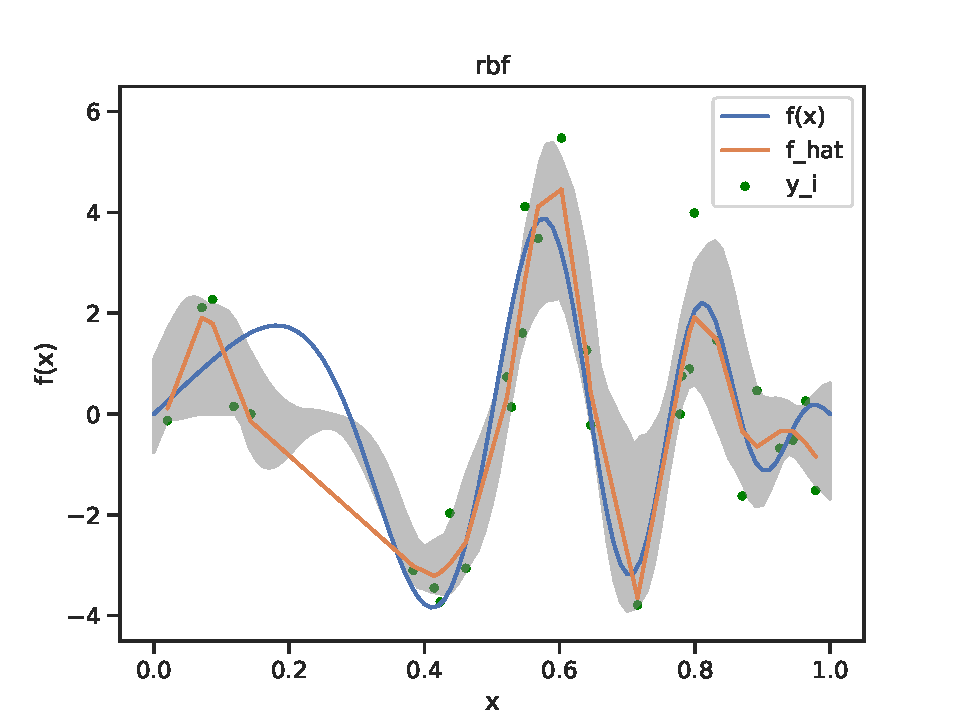
\includegraphics[width=.9\textwidth]{{hw3/30_rbf}.pdf}
\end{center}


\begin{center}
    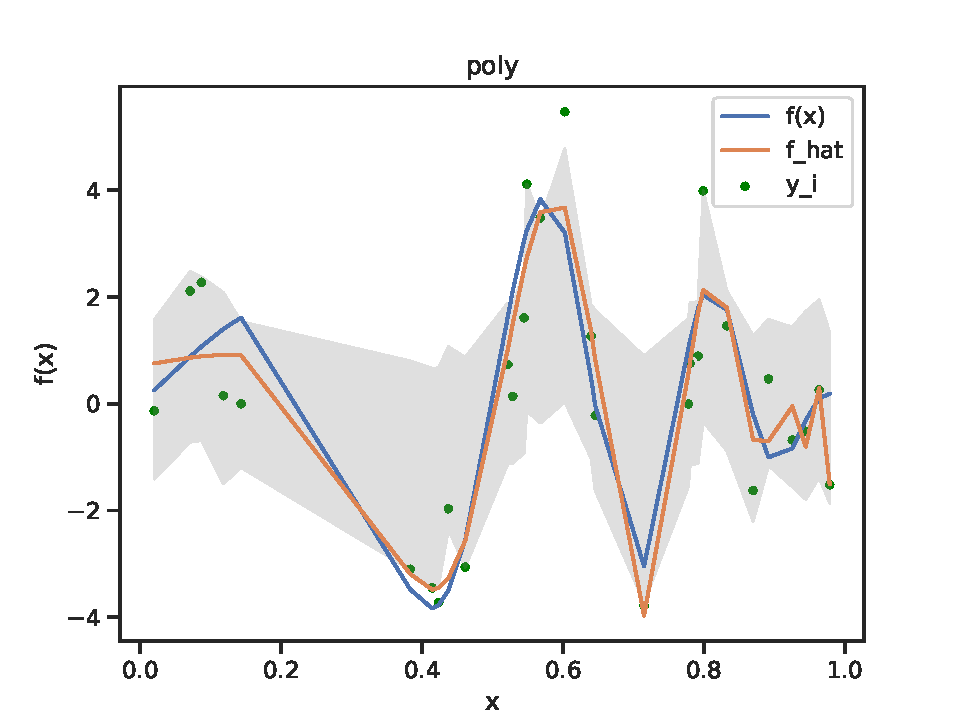
\includegraphics[width=.9\textwidth]{{hw3/30_poly}.pdf}
\end{center}

\begin{center}
    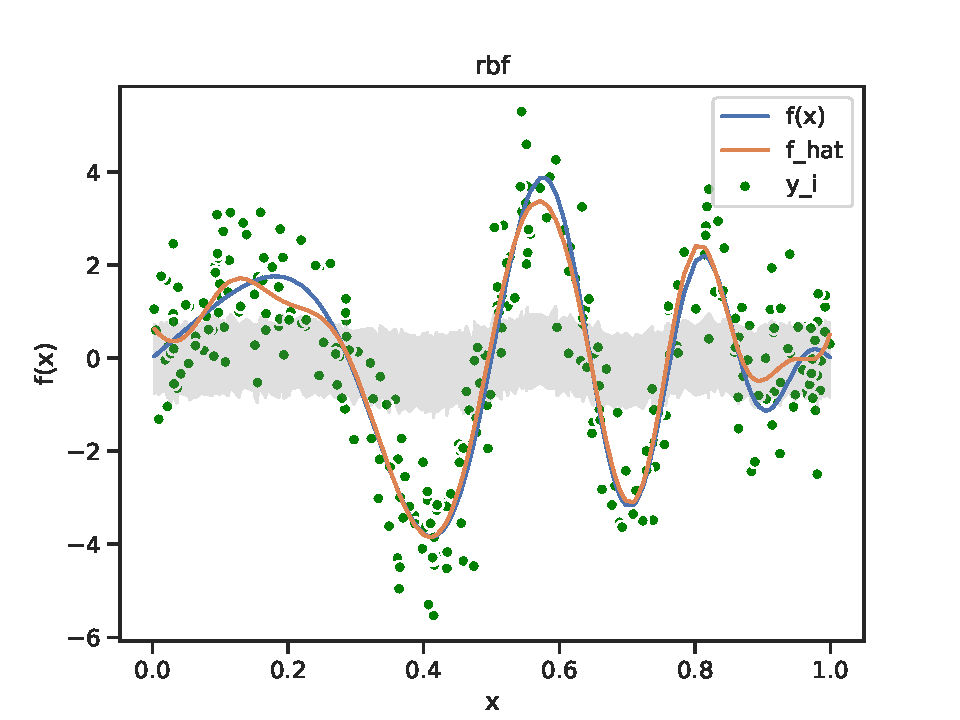
\includegraphics[width=.9\textwidth]{{hw3/300_rbf}.pdf}
\end{center}


\begin{center}
    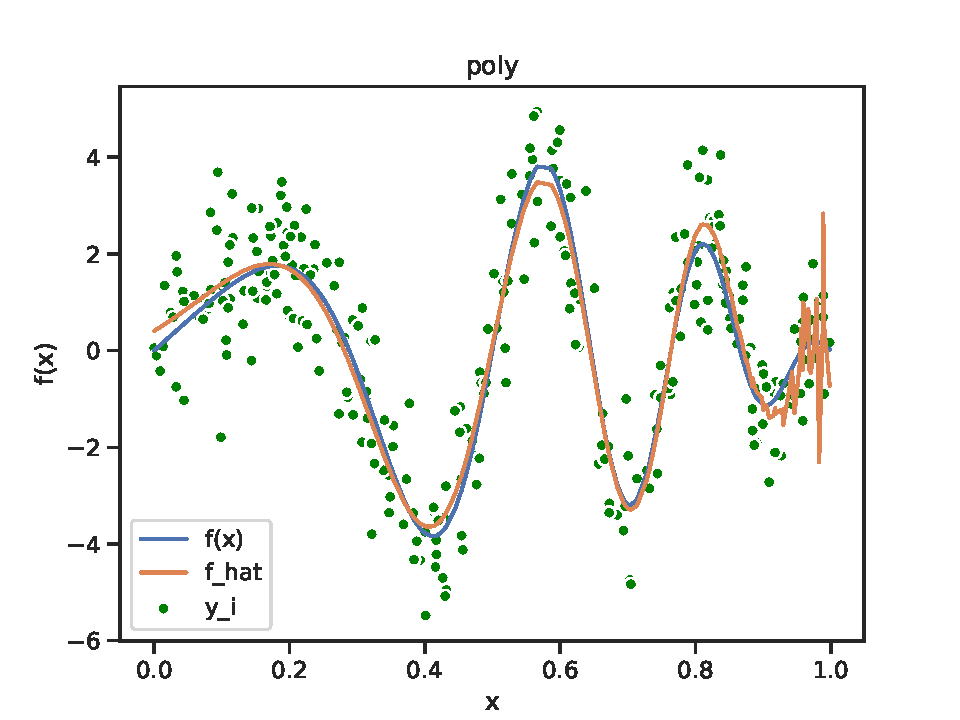
\includegraphics[width=.9\textwidth]{{hw3/300_poly}.pdf}
\end{center}


\section*{Problem 3 d}

See sections a, b, and c. I have included the results there. 

\section*{Problem 3 e}

\section*{Problem 3 code}

\lstinputlisting[language=python]{hw3/kernel.py}

















\newpage







\section{$k$-means clustering}

4. \grade{5} Given a dataset $x_1,..., x_n \in \R^{d}$ and an integer $1 \leq k \leq n$, recall the following $k$-means objective function
\begin{align}
    \min_{\pi_1, ..., \pi_k} \sum_{i=1}^{k} \sum_{j \in \pi_i} \norm{ x_j - \mu_{i} }^2_2 \ , \quad \mu_i = \frac{1}{|\pi_i|} \sum_{j \in \pi_i} x_j \ . \label{eq:kmeans_obj}
\end{align}
Above, $\{\pi_i\}_{i=1}^{k}$ is a partition of $\{1, 2, ..., n\}$. The objective \eqref{eq:kmeans_obj} is NP-hard\footnote{
To be more precise, it is both NP-hard in $d$ when $k=2$ and $k$ when $d=2$.
See the references on the wikipedia page for $k$-means for more details.
} to find a global minimizer of. Nevertheless the commonly used heuristic which we discussed in lecture, known as Lloyd's algorithm, typically works well in practice.
Implement Lloyd's algorithm for solving the $k$-means objective \eqref{eq:kmeans_obj}.
Do not use any off the shelf implementations, such as those found in \texttt{scikit-learn}.
\begin{enumerate}
    \item Run the algorithm on MNIST with $k=5,10,20$, plotting the objective function \eqref{eq:kmeans_obj} as a function of iteration. Visualize (and include in your report) the cluster centers as a $28\times 28$ image.
    \item Implement the \texttt{kmeans++} initialization scheme\footnote{See \url{http://ilpubs.stanford.edu:8090/778/1/2006-13.pdf}.} for your
        $k$-means implementation and repeat part a.  Note that this initialization scheme is widely used in practice, and as a rule should be used. Plot the objective function as a function of iteration. Are the identified centers visually better than part a? 
\end{enumerate}





\newpage

\section*{Problem 4 a Answer}

\begin{center}
    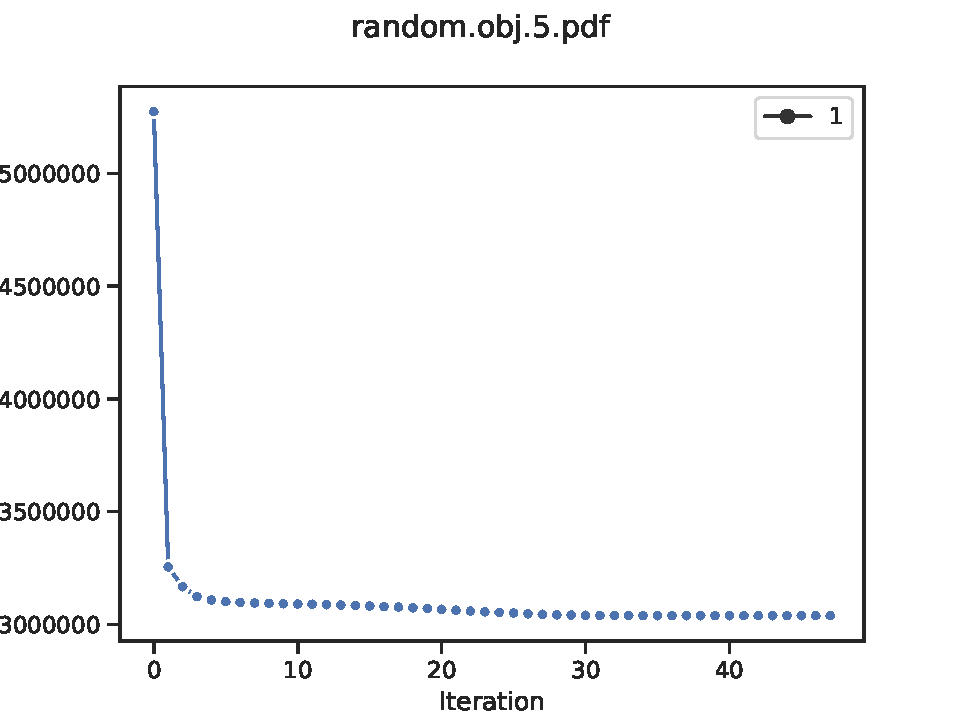
\includegraphics[width=.9\textwidth]{{hw3/random.obj.5}.pdf}
\end{center}

\begin{center}
    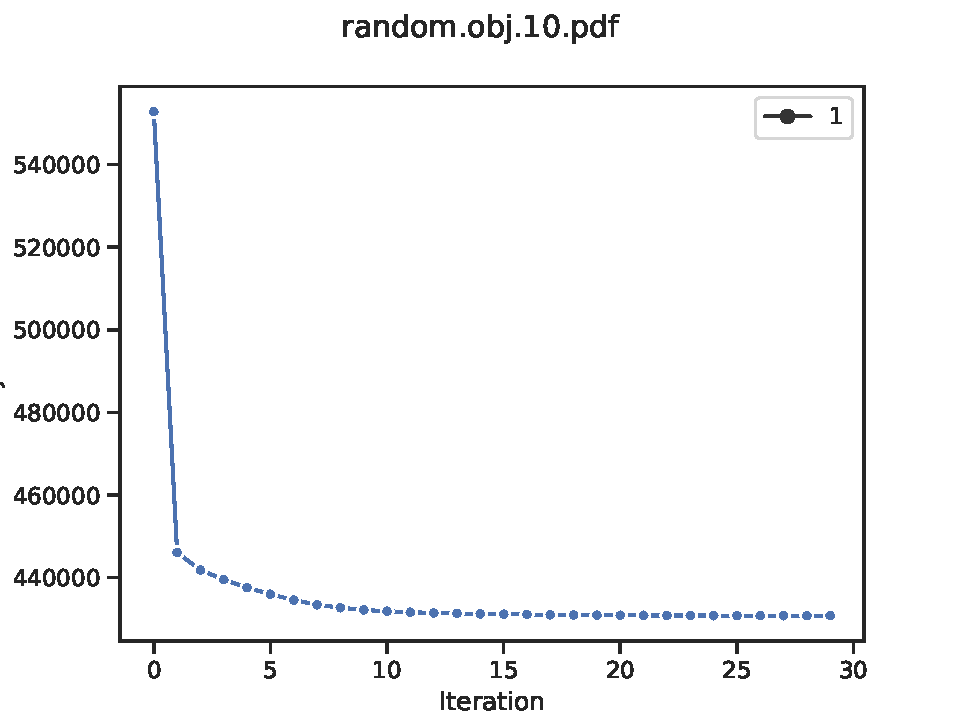
\includegraphics[width=.9\textwidth]{{hw3/random.obj.10}.pdf}
\end{center} 

\begin{center}
    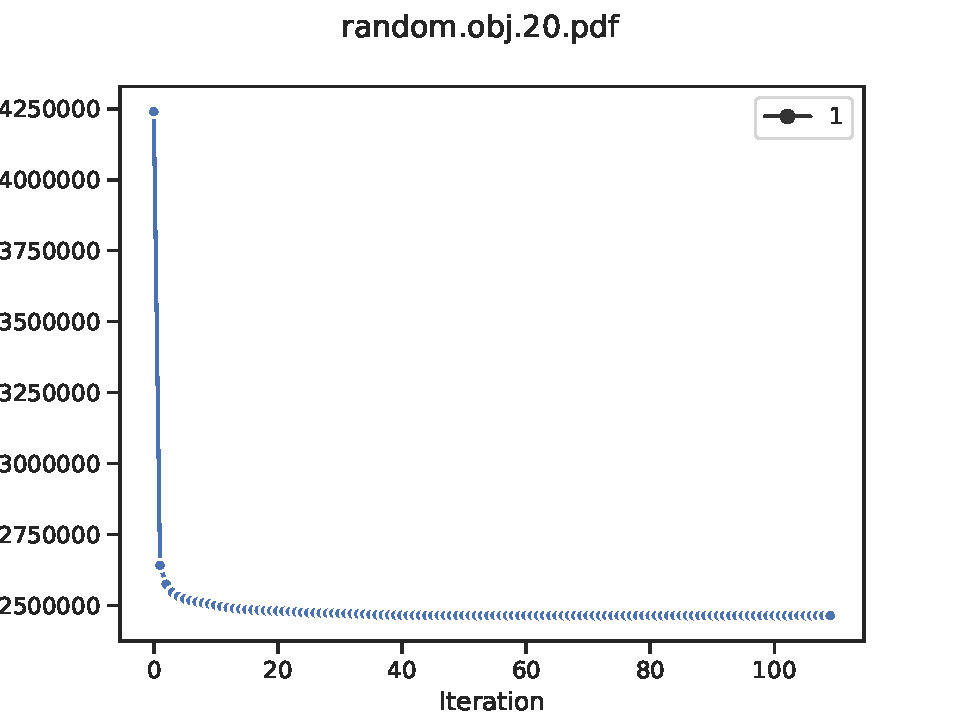
\includegraphics[width=.9\textwidth]{{hw3/random.obj.20}.pdf}
\end{center}


\begin{center}
    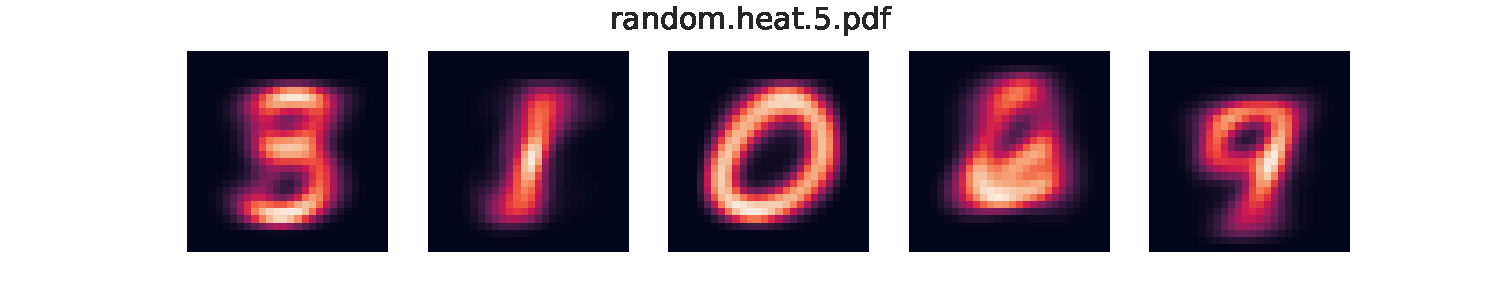
\includegraphics[width=.9\textwidth]{{hw3/random.heat.5}.pdf}
\end{center}

\begin{center}
    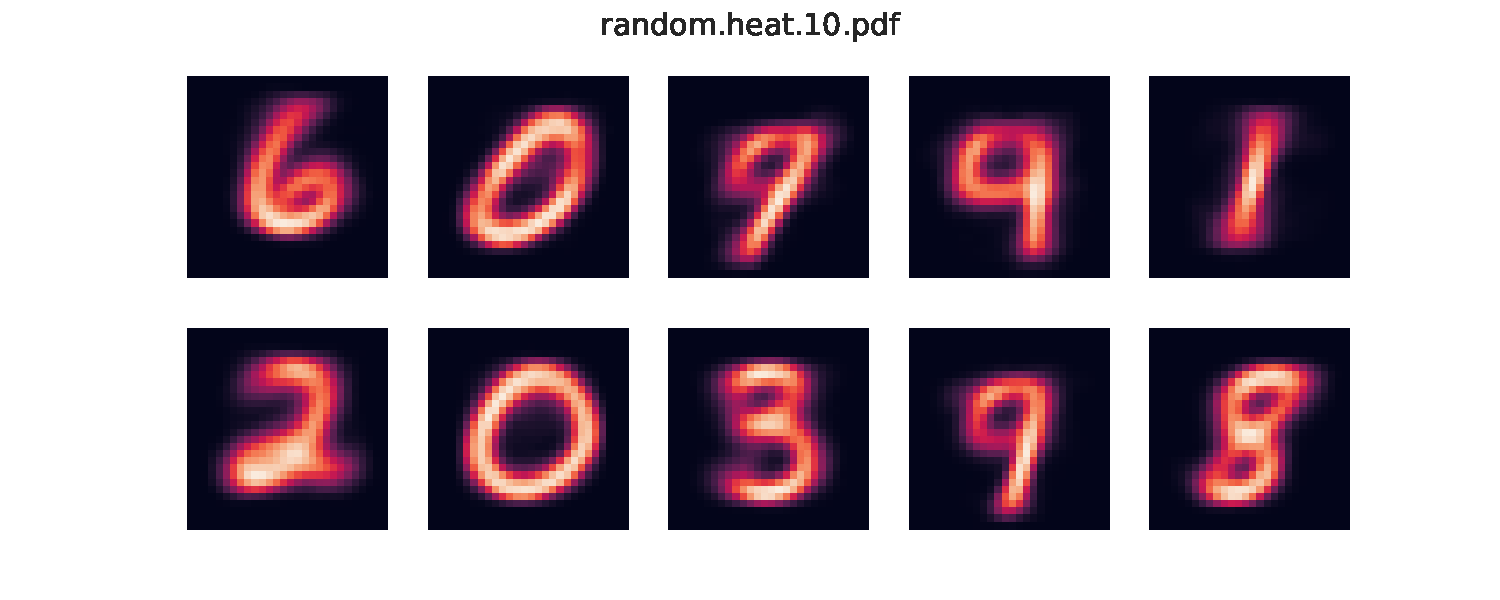
\includegraphics[width=.9\textwidth]{{hw3/random.heat.10}.pdf}
\end{center} 

\begin{center}
    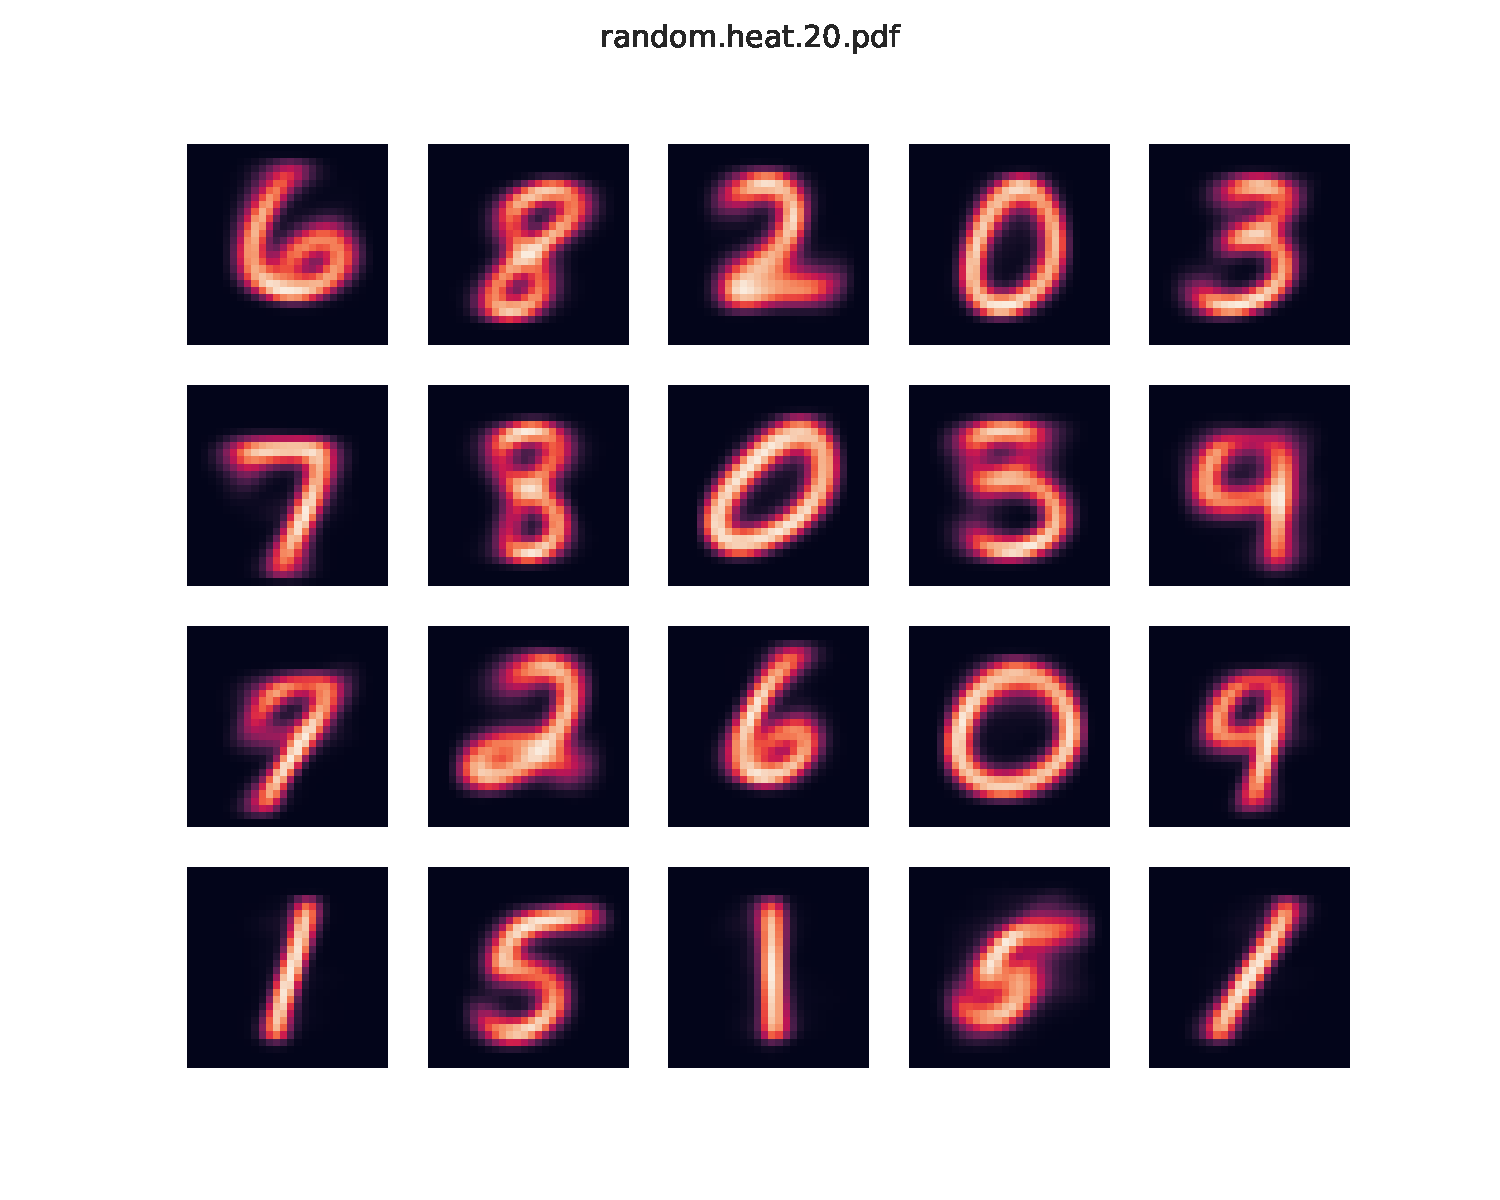
\includegraphics[width=.9\textwidth]{{hw3/random.heat.20}.pdf}
\end{center}


\section*{Problem 4 b Answer}

I would not say the cluisters look vizually much better with the kmeans ++ scheme. However, they look at least as good, and on average converge in significantly fewer iterations than the random initialization.

\begin{center}
    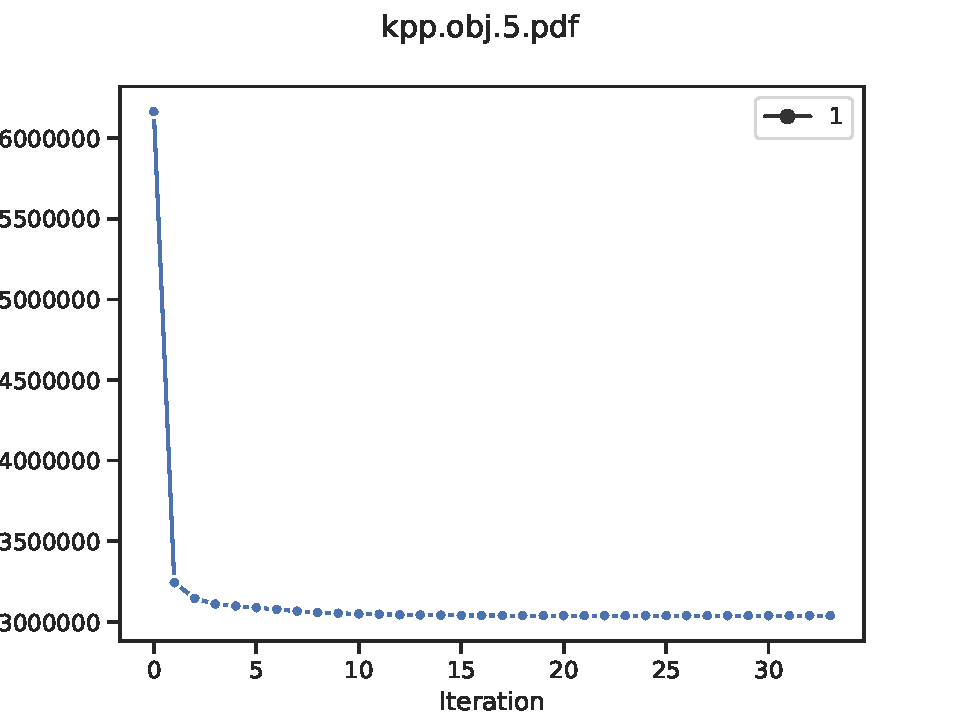
\includegraphics[width=.9\textwidth]{{hw3/kpp.obj.5}.pdf}
\end{center}

\begin{center}
    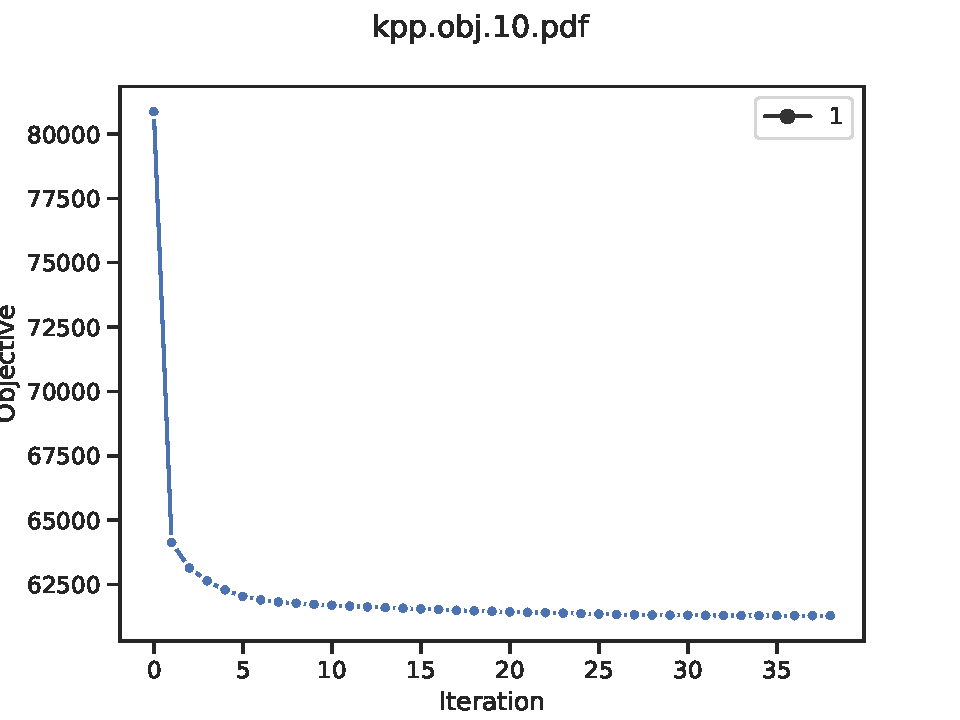
\includegraphics[width=.9\textwidth]{{hw3/kpp.obj.10}.pdf}
\end{center} 

\begin{center}
    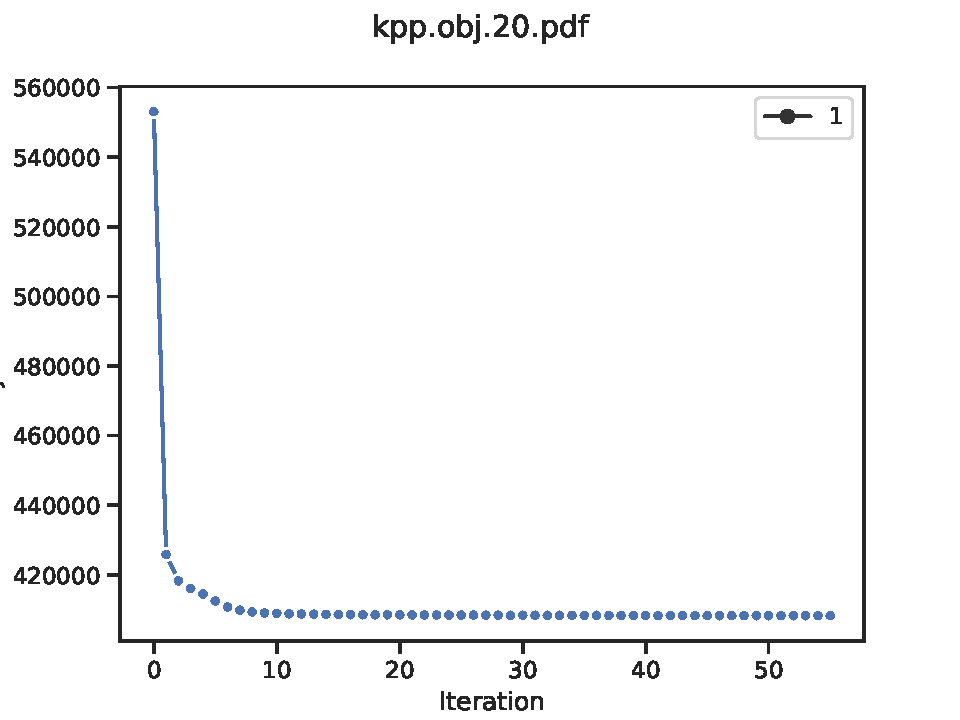
\includegraphics[width=.9\textwidth]{{hw3/kpp.obj.20}.pdf}
\end{center}


\begin{center}
    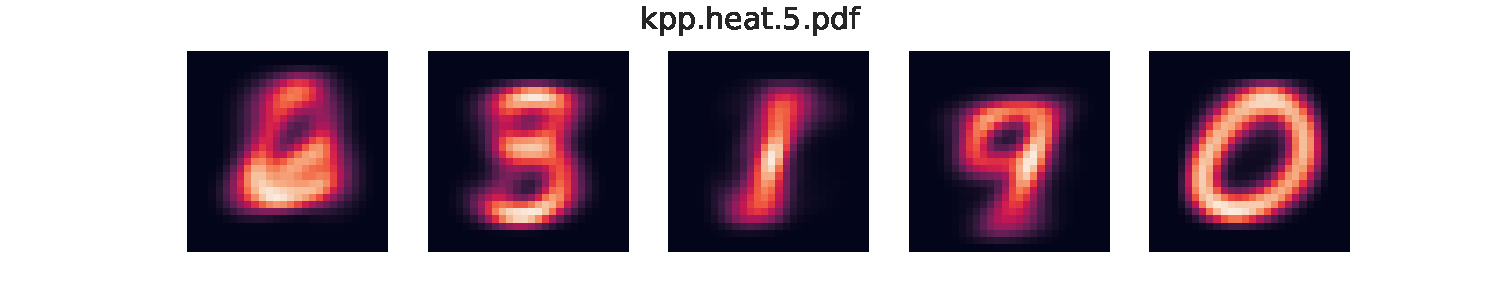
\includegraphics[width=.9\textwidth]{{hw3/kpp.heat.5}.pdf}
\end{center}

\begin{center}
    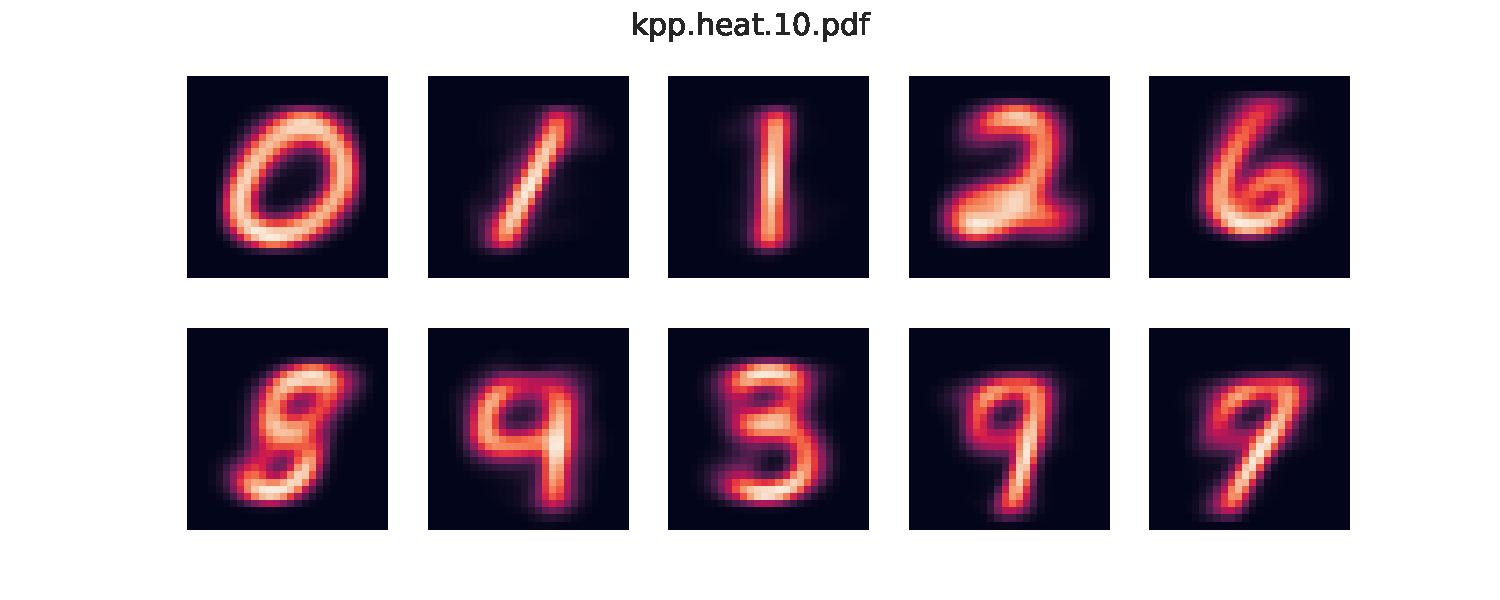
\includegraphics[width=.9\textwidth]{{hw3/kpp.heat.10}.pdf}
\end{center} 

\begin{center}
    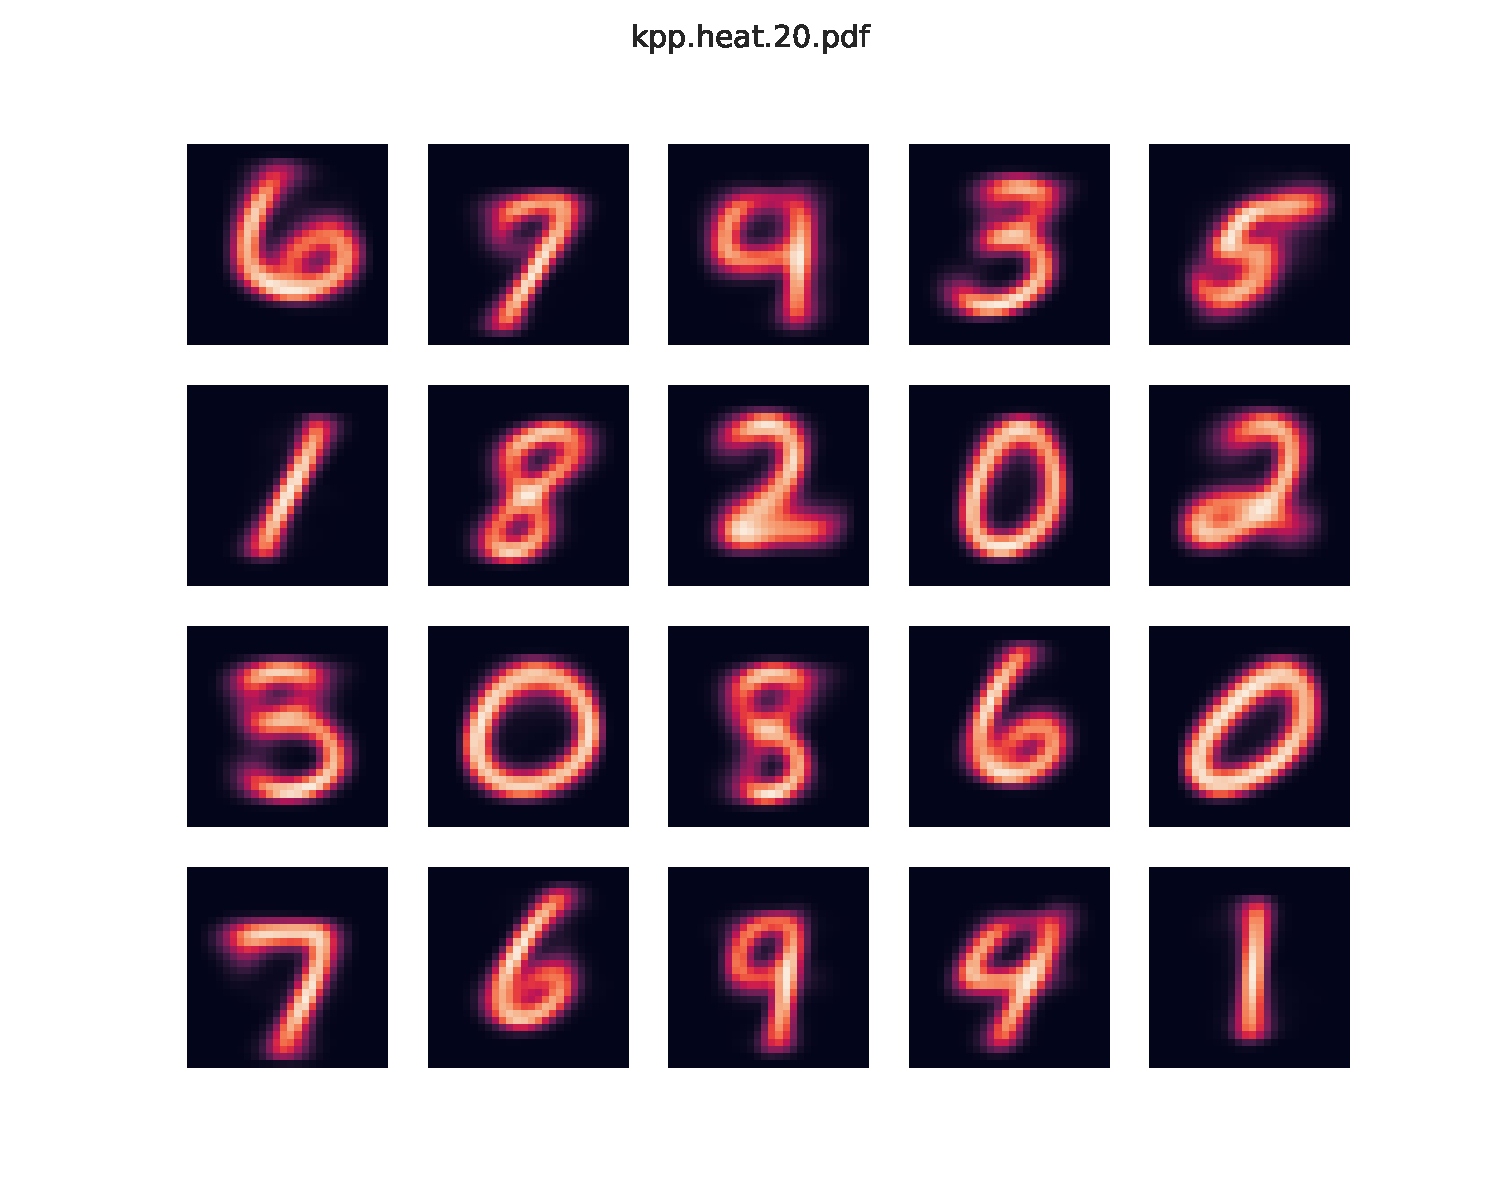
\includegraphics[width=.9\textwidth]{{hw3/kpp.heat.20}.pdf}
\end{center}


\section*{Problem 4 code}

\lstinputlisting[language=python]{hw3/kmeans.py}

\newpage




















\section{Joke Recommender System}

5. \grade{8} You will build a personalized joke recommender system. There are $m = 100$ jokes and $n = 24,983$ users\footnote{Data from \url{http://eigentaste.berkeley.edu/dataset/}}. As historical data, every user read a subset of jokes and rated them. The goal is to recommend more jokes, such that the recommended jokes match the individual user's sense of humor.
The historical rating is represented by a matrix $R\in \R^{n \times m}$. The entry $R_{i,j}$ represents the user $i$'s rating on joke $j$. The rating is a real number in $[-10,10]$: a higher value represents that the user is more satisfied with the joke.
The directory $\tt /jokes$ contains the text of all $100$ jokes. Read them before you start! In addition, you are provided with two files:
\begin{itemize}
\item $\tt train.txt$ contains the joke-user-score data representing the training set. Each line takes the form ``$\tt i,j,s$'', where $\tt i$ is the user index, $\tt j$ is the joke index, and $\tt s$ is the user's score in $[-10,10]$ describing how much they liked the joke (higher is better).
\item $\tt test.txt$ has the same format, with the same users rating movies held out from the training set.
\end{itemize}

Latent factor model is the state-of-the-art method for personalized recommendation. It learns a vector representation $u_i\in \R^d$ for each user and a vector representation $v_j\in \R^d$ for each joke, such that
the inner product $\langle u_i,v_j\rangle$ approximates the rating~$R_{i,j}$. You will build a simple latent factor model.
We will evaluate our learnt vector representations by two metrics
\begin{itemize}
  \item Mean squared error: $\frac{1}{|S|} \sum_{(i,j)\in S} (\langle u_i,v_j\rangle - R_{ij})^2$ where $S$ (and the corresponding $R_{i,j}$ values) are from the test set
  \item Mean absolute error: $\frac{1}{n} \sum_{i=1}^n \frac{1}{|\mathcal{N}_i|} \sum_{j \in \mathcal{N}_i} |\langle u_i,v_j\rangle - R_{ij}|$ where $\mathcal{N}_i$ are the jokes rated by user $i$ in the test set
\end{itemize}  

You will implement multiple estimators and use the inner product $\langle u_i,v_j\rangle$ to predict if user $i$ likes joke $j$ in the test data.
You will choose hyperparameters like $d$ or the amount of regularization by creating a validation set from the training set.

\begin{enumerate}
\item The first estimator pools all the users together and just predicts what the average user in the training set rated the joke. This is equivalent to $d=1$ with $u$ as the all ones vector and $v$ minimizing least squares.    

\item Now replace all missing values in $R_{i,j}$ no in the training set by zero. Then use singular value decomposition (SVD) to learn a lower dimensional vector representation for users and jokes. Recall this means to project the data vectors to lower dimensional subspaces of their corresponding spaces, spanned by singular vectors. Refer to the lecture materials on SVD, PCA and dimensionality reduction. You should use an efficient solver, I recommend \texttt{scipy.sparse.linalg.svds}. Try $d=1,2,5,10,20,50$ and plot the error metrics on the train and test as a function of $d$. 

\item For sparse data, replacing all missing values by zero is not a completely satisfying solution. A missing value means that the user has not read the joke, but doesn't mean that the rating should be zero. A more reasonable choice is to minimize the MSE only on rated jokes. Let's define a loss function:
\[
  L\Big(\{u_i\},\{v_j\}\Big) := \sum_{(i,j)\in T} (\langle u_i,v_j\rangle - R_{i,j})^2
  + \lambda \sum_{i=1}^n \|u_i\|_2^2 + \lambda \sum_{j=1}^m \|v_j\|_2^2,
\]
where $T$ and $R_{i,j}$ here are from the training set and $\lambda > 0$ is the regularization coefficient. Implement an algorithm to learn vector representations by minimizing the loss function $L(\{u_i\},\{v_j\})$.
Try $d=1,2,5,10,20,50$ and plot the error metrics on the train and test as a function of $d$. 
Note that you may need to tune the hyper-parameter $\lambda$ to optimize the performance.

{\bf Hint:} you may want to employ an alternating minimization scheme. First, randomly initialize $\{u_i\}$ and $\{v_j\}$. Then minimize the loss function with respective to $\{u_i\}$ by treating $\{v_j\}$ as constant vectors, and minimize the loss function with respect to $\{v_j\}$ by treating $\{u_i\}$ as constant vectors. Iterate these two steps until both $\{u_i\}$ and $\{v_j\}$ converge. Note that when one of $\{u_i\}$ or $\{v_j\}$ is given, minimizing the loss function with respect to the other part has closed-form solutions. You should never be allocating an $m \times n$ matrix for this problem. 


\end{enumerate}





















\section*{Problem 5 a Answer}

Part A train:   MSE:24.870751120670207	MAE:4.114762091223429 \\
Part A test:	MSE:24.867391804873332	MAE:4.114205038713316 \\

\section*{Problem 5 b Answer}
\begin{center}
    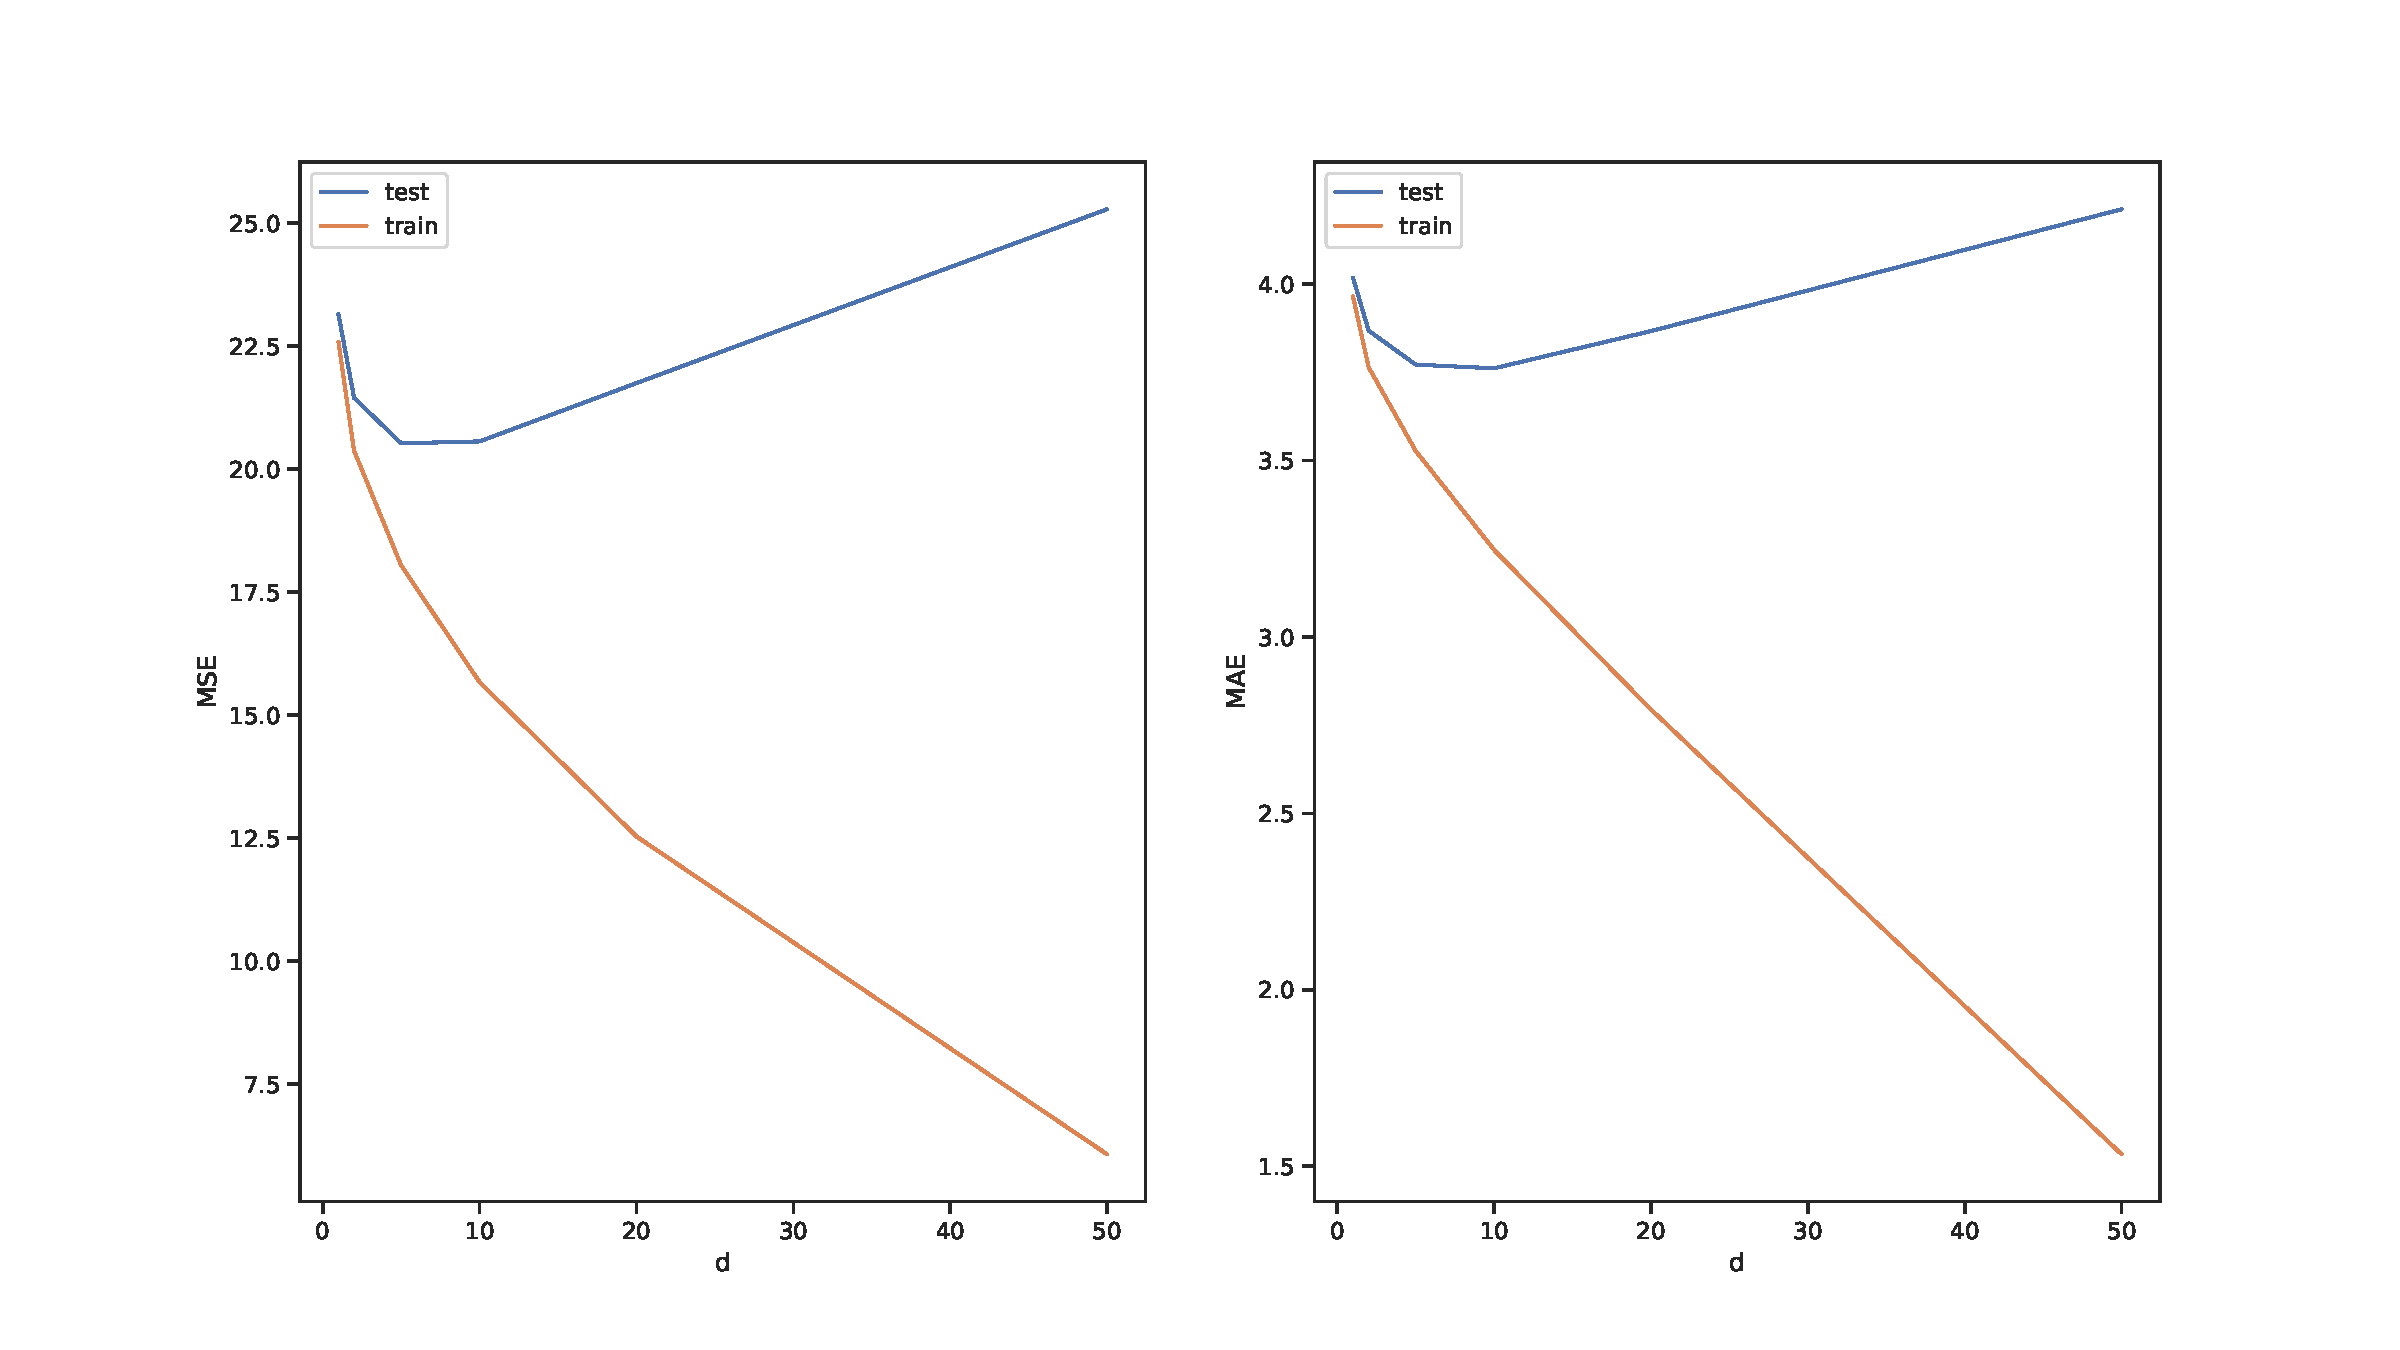
\includegraphics[width=.9\textwidth]{hw3/5b.pdf}
\end{center}

\section*{Problem 5 c Answer}

\begin{center}
    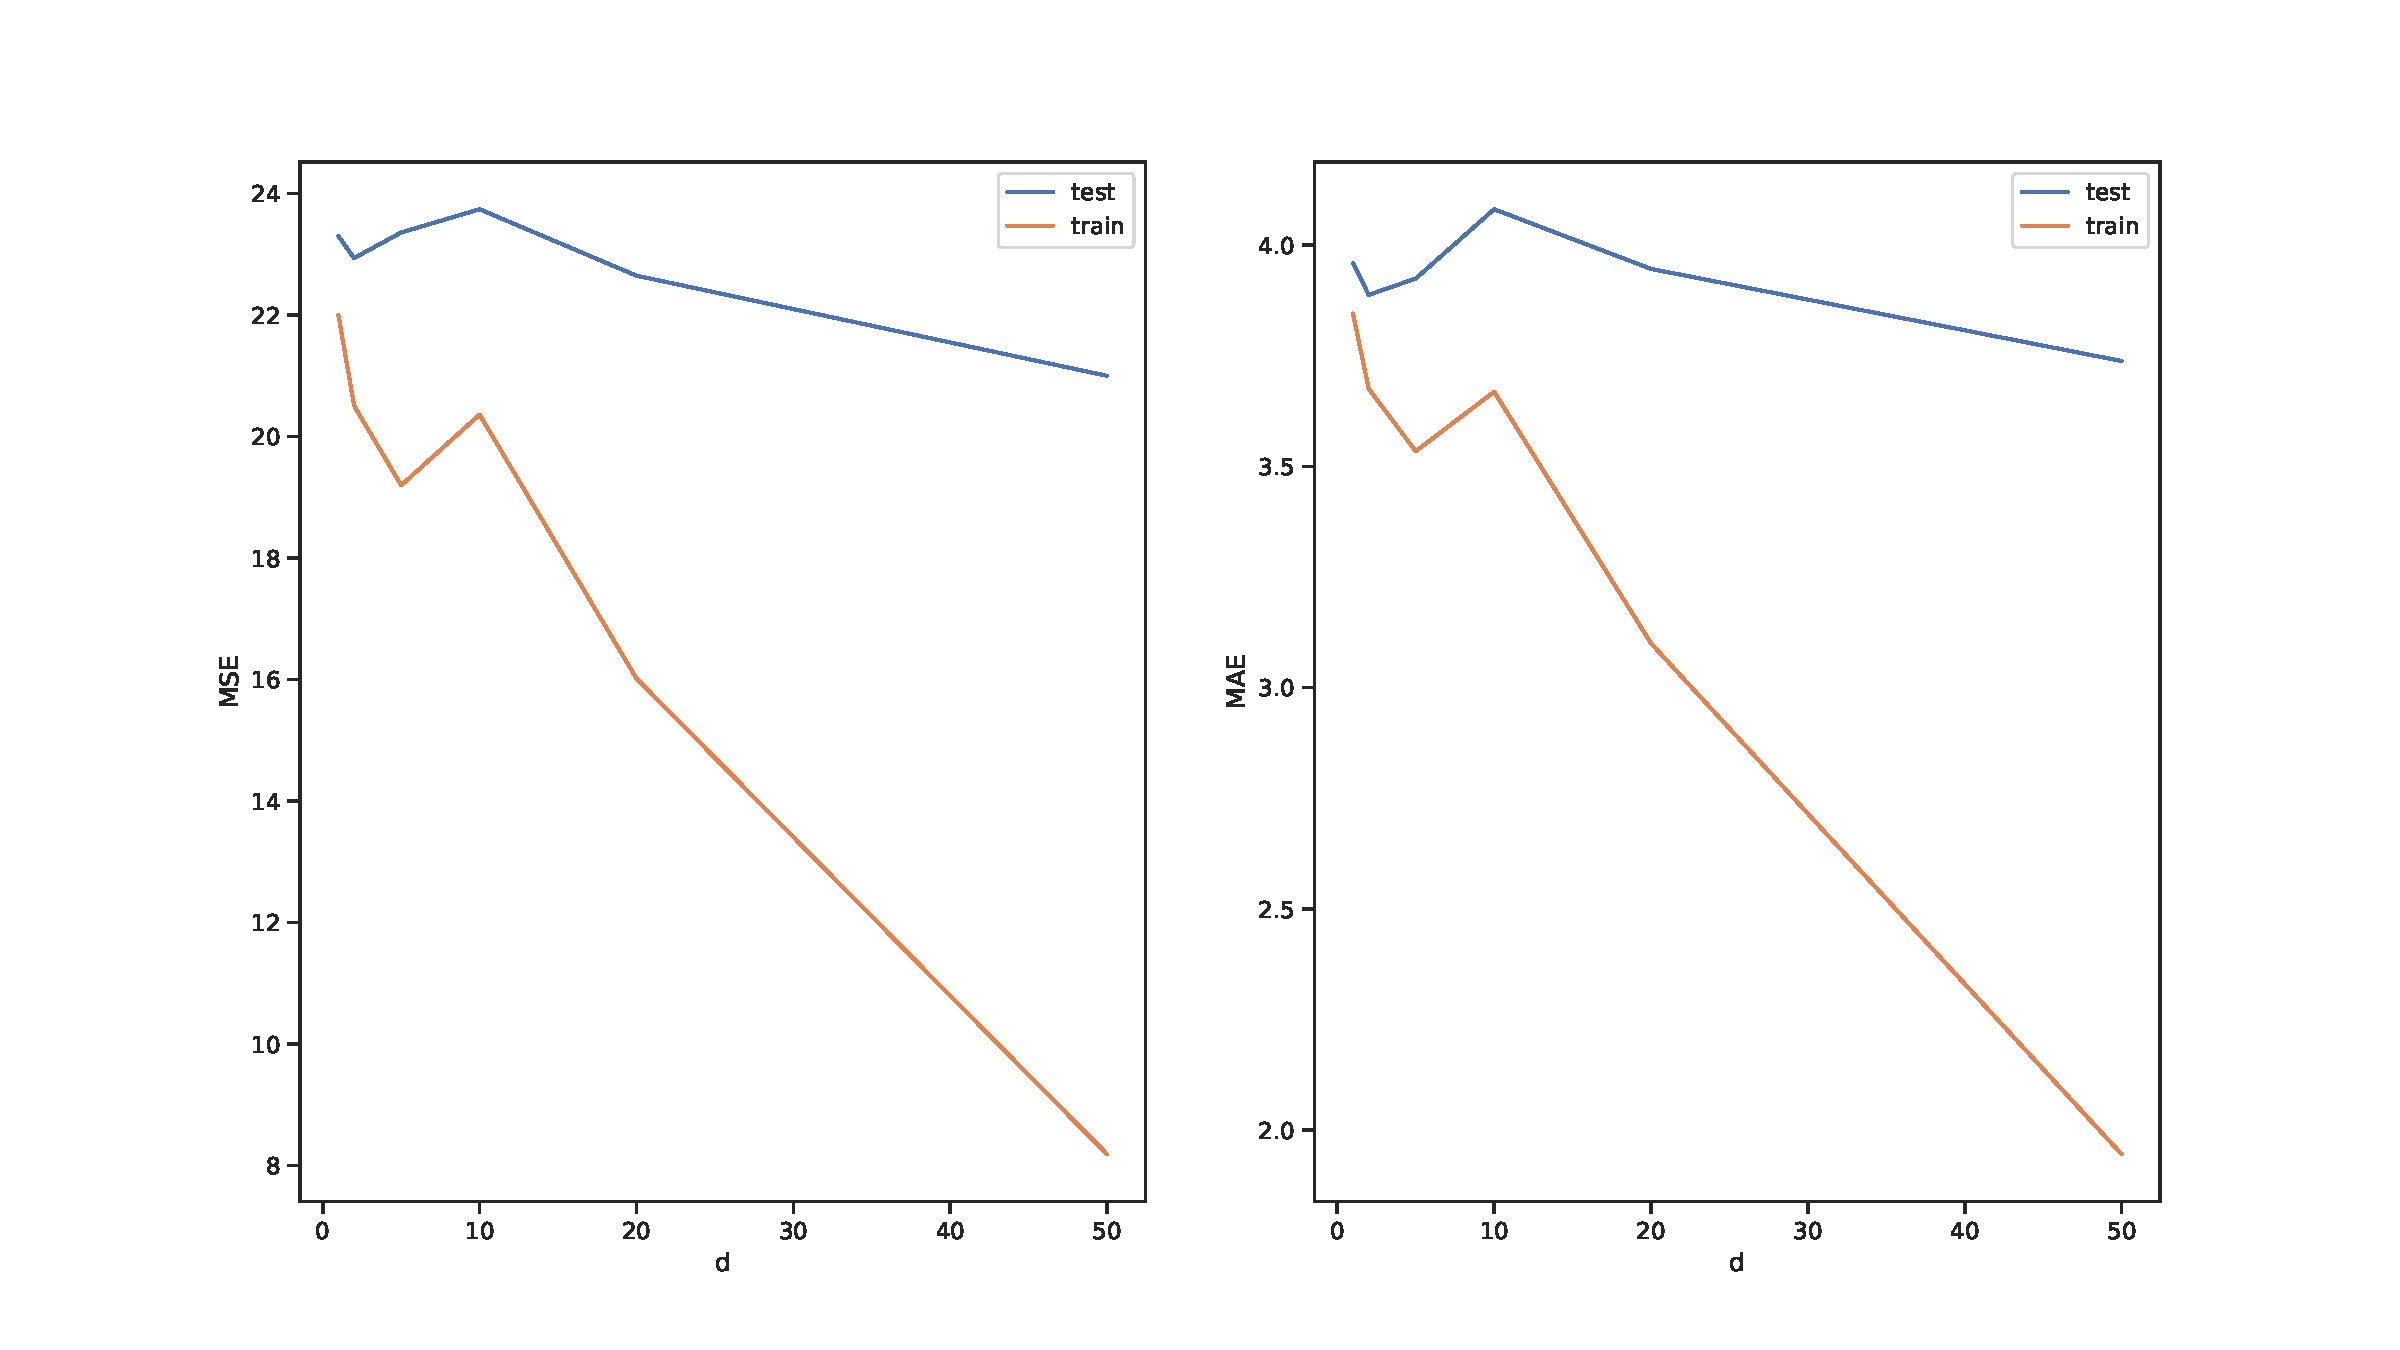
\includegraphics[width=.9\textwidth]{hw3/5c.pdf}
\end{center}

I choose to optimize $U$ and $V^T$ iteritavly as suggested in the hint. $U$ and $V^T$ were initialized randomly using a normal distribution. Additionally I made a validation set to choose all the $\lambda$s reported below. Plotted above is the MSE and MAE. 


The MSE, MAE from the test set followed by d, and the validation set determined lambda $\lambda$ \\
23.133794962901547 3.907912362195389 1 0.01 \\
23.471354590976414 3.928374180881678 2 1.0 \\
23.72090424658509 3.955840161002923 5 10.0 \\
23.89584521011899 4.092839006672779 10 100.0 \\
22.294961993106273 3.905808727356969 20 100.0 \\
20.086316023858192 3.6368761845264865 50 100.0 \\



\section*{Problem 5 code}

\lstinputlisting[language=python]{hw3/jokes.py}


\end{document}
